\section{Segmentation of the MILP problem}
\label{section:segment}
In this section we propose a preprocessing pipeline that makes the problem more scalable. Alg. \ref{alg:outline} shows the outline of the algorithm.
\begin{algorithm}
\caption{General outline}
\label{alg:outline}
\begin{algorithmic}[1]
\State $T \leftarrow \{\}$ \Comment{The list of solved subtrajectories}
\State $path \leftarrow$ \Call{Theta*}{$scenario$}
\State $events \leftarrow$ \Call{FindTurnEvents}{$path$}
\State $segments \leftarrow$ \Call{GenSegments}{$path$, $events$}
\ForEach {$segment \in segments$}
\State \Call{UpdateStartState}{$segment$}
\State \Call{GenSafeRegion}{$scenario$, $segment$}
\State \Call{GenSubMILP}{$scenario$, $segment$}
\State $T \leftarrow T \cup \{$ \Call{SolveSubMILP}{} $\}$
\EndFor
\State $result \leftarrow $\Call{MergeTrajectories}{$T$}
\end{algorithmic}
\end{algorithm}

First, we find an initial path with the Theta* algorithm (line 2). Unlike a trajectory, a path is not time-dependent and does not take dynamic properties into account. Then, we find all the turns in that path (line 3). After that, we generate path segments based on those turns (line 4). Each path segment contains the information needed to construct a MILP subproblem. Finally, for each segment, a MILP subproblem is constructed and solved (line 8-9). Before the MILP subproblem is solved, a heuristic selects several obstacles to be modeled in the problem. A genetic algorithm generates a convex safe region which is allowed to overlap those selected obstacles only (line 7). Because the UAV must stay within the safe region, it cannot collide with obstacles. For all but the first segment, the starting state for the UAV in the MILP problem is updated to match the final state of the UAV in the previous segment (line 6). Once all the segments have been solved, their trajectories are merged into the final result (line 11).\\
Our goal is to divide the problem into subproblems so that only a minimal number of obstacles need to be modeled in each subproblem, while still resulting in a relatively fast trajectory. Subproblems based on shorter segments with fewer obstacles are easier to solve, but the UAV will need to travel at a lower velocity. This is because there is no information available about the next segment. 
If the next segment contains a tight turn, the UAV may not be able to slow down enough if it is going too fast. Longer segments allow the UAV to travel faster, but they need more time to solve.\\
For the best results, we want to find segments which are as large as possible but contain as few obstacles as possible. By generating a segment for each turn in the Theta* path, we can make the segments just large enough so the UAV can always slow down in time to execute the turn. This way the UAV will always turn efficiently, without making the segments too large to solve in an acceptable amount of time.
\subsection{Finding the initial path}
\begin{figure}
    \centering
        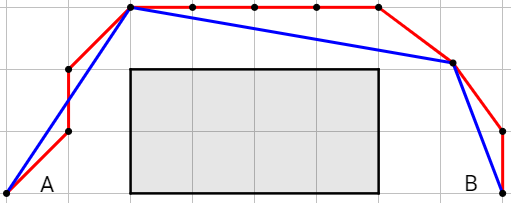
\includegraphics[width=0.65\columnwidth]{img/a_theta_star_comp3}
    \caption{A typical A* path in blue compared to a Theta* path in red. The gray rectangle is an obstacle.}\label{fig:pre-comp}
\end{figure}

\begin{figure}[!t]
    \centering
        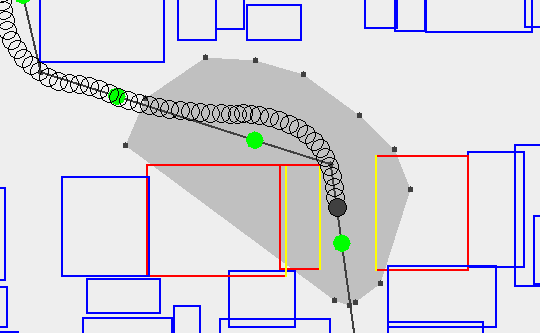
\includegraphics[width=0.7\columnwidth]{img/pre-full}
    \caption{The red/yellow shapes are the obstacles modeled in the MILP problem, using the same color scheme as in Fig. \ref{fig:obs-clear}. The blue shapes are the remaining obstacles. The green circles depict the transitions between segments. The dark gray shape is the convex safe area generated by the genetic algorithm. The solid black circle represents the current position of the UAV, with the hollow circles showing the position in previous time steps.}\label{fig:pre-full}
\end{figure}
The first step in Alg. \ref{alg:outline} is finding the Theta* path (line 2), which will be used to divide the problem into segments. The MILP problem generated from each segment needs an intermediate goal to guide the UAV closer the final goal position.\\
We use Theta* \cite{Daniel2010} to find an initial path which connects the start and goal positions. Theta* is a variant of A* which eliminates the jagged paths associated with A* as demonstrated in Fig. \ref{fig:pre-comp}.
This path does not take any of the vehicle dynamics into account. Multirotor UAVs can hover, so the UAV can always follow this path by moving in straight lines and stopping at each node of the path. This ensures that successful navigation to the goal position is possible.\\

\subsection{Detecting turn events}
Because the shortest path between two points in Euclidian geometry is a straight line, any turn at a node in the Theta* path must have at least one obstacle on the inside of that turn. A turn without an obstacle on the inside can always replaced by a shorter, straight line segment. This means that by definition these "inner" obstacles make the search space non-convex. A shape is convex if every point on the line between any two points inside the shape is also inside the shape. Because moving in a straight line between two valid positions on either side of the turn is not possible, the search space must be non-convex if turns in the Theta* path exist.\\
Non-convexity of the search space is the main cause for the poor performance of Mixed Integer Programming \cite{Deits2015}. We have shown that the turns in the path correspond with parts of the problem which must be non-convex. Because of this, we have chosen to generate the segments such that there is at most a single turn in each segment. This limits the non-convexity for each subproblem, significantly improving execution time.\\
In some cases, a Theta* path contains multiple nodes for a single turn. Alg. \ref{alg:corners} groups those nodes together into turn events.

\begin{algorithm}
\caption{Finding Turn Events}
\label{alg:corners}
\begin{algorithmic}[1]
\Function{FindTurnEvents}{$path$}
  \State $\Delta max \leftarrow$ max. acc. distance * turn tolerance
  \State $events \leftarrow \{\}$ \Comment{The list of turn events found so far}
  \State $i \leftarrow 1$ \Comment{Skip the start node, it can't be a turn}
  \While{$i < |path| - 1$ } \Comment{Skip the goal node}
  	\State $event \leftarrow \{ path(i) \}$ \Comment{Start new turn event}
  	\State $turnDir \leftarrow$ \Call{TurnDir}{$path(i)$} 
    	\State $i \leftarrow  i + 1$
    	\While{$i < |path| - 1$ }
    	\If{$||path(i-1) - path(i)|| > \Delta max$}
    		\Break \Comment{Node is too far from previous}
	\EndIf
	\If{\Call{TurnDir}{$path(i)} \neq turnDir$}
		\Break \Comment{Node turns in wrong direction}
	\EndIf
	\State $event \leftarrow event \cup \{ path(i) \}$\Comment{Add to event}
	\State $i \leftarrow  i + 1$
	
    	\EndWhile
    	
    	\State $events \leftarrow events \cup \{ event \}$
  \EndWhile
\Return $events$
\EndFunction
\end{algorithmic}
\end{algorithm}
In the Theta* path, all but the first and last nodes are turns in the path. The second node is always the first node in a new turn event (line 5). Subsequent nodes in the path which are not too far away from the previous node (line 9) and turn in the same direction (line 12) are added to the current turn event (line 15). The maximum distance between nodes in the same turn depends on the maximum acceleration distance of the UAV and a turn tolerance parameter (line 2). The maximum acceleration distance is the distance the UAV needs to accelerate from zero to its maximum velocity, or slow down from the maximum velocity to zero. Once a node is found which does not belong in the event, the event is stored (line 18), a new event is created for that node (line 5) and the process repeats until no more nodes are left.
\subsection{Generating path segments}
\begin{algorithm}
\caption{Generating the segments}
\label{alg:segments}
\begin{algorithmic}[1]
\Function{GenSegments}{$path$, $events$}
\State $segments \leftarrow \{\}$
\State $catchUp \leftarrow true$
\State $lastEnd \leftarrow path(0)$
\For {$i \gets 0, |events| - 1 $}
\State $event \leftarrow events(i)$
\If{$catchUp$}
	%\State $segStart \leftarrow $ \Call{ExpandBackw}{$event.start$}
	%\State \Call{AddSegments}{$lastSegEnd$, $segStart$}
	%\State $lastSegEnd \leftarrow segStart$ 
	\State expand $event.start$ backwards
	\State add segments from $lastEnd$ to $event.start$
	\State $lastEnd \leftarrow event.start$
\EndIf
\State $nextEvent \leftarrow events(i+1)$
\If{$nextEvent.start$ is close to $event.end$}
	\State $mid \leftarrow$ middle between $event$ \& $nextEvent$
	\State add segment from $lastEnd$ to $mid$
	\State $lastEnd \leftarrow mid$
	\State $catchUp \leftarrow false$
\Else
	\State expand $event.end$ forwards
	\State add segment from $lastEnd$ to $event.end$
	\State $lastEnd \leftarrow event.end$
	\State $catchUp \leftarrow true$
\EndIf
\EndFor
\State add segments from $lastEnd$ to $path(|path|-1)$
\Return $segments$
\EndFunction
\end{algorithmic}
\end{algorithm}
Each path segment contains the information needed to construct a MILP subproblem. Alg. \ref{alg:segments} constructs the segments using turn events.
Each segment needs to be large enough so the UAV can safely approach and exit each turn. A multirotor UAV can always safely navigate a turn if it can come to a complete stop before the turn. That is satisfied if the segment starts at least the maximum acceleration distance away from the turn. If the segment starts even earlier, the UAV has more space to maneuver and can navigate the turn more efficiently. However, as the segment gets larger, so does the difficulty of the segment. The approach margin multiplier determines the expansion distance around turn events, based on the maximum acceleration distance. \\
To generate the segments, Alg. \ref{alg:segments} considers each turn event in turn. It keeps track of the end point of the last segment it generated with $lastEnd$. When constructing a segment, it considers the distance between the end of the current turn event and the start of the next turn event. On line 13, two events are too close to each other if they are separated by less than three times \footnote{Requiring three (instead of two) times the expansion distance as separation between turn events ensures that the segment between those turns is also at least as long as the expansion distance. This prevents some issues that can occur with very short segments.} the expansion distance. In that case, the segment is constructed to end in the middle between the current and next event (line 14-16). If the events are far enough apart, the end of the current event is expanded forwards by the full expansion distance(line 19-21). Because the next turn event is a long distance away, the $catchUp$ flag is set to true (line 22), ensuring that one or more segments are added to catch up to the start of the next event (line 7-10). To limit the size of segments, they can be no longer than the distance the UAV can travel at maximum velocity in $T_{max}$ time.
\subsection{Generating the safe region for each segment}
\begin{algorithm}
\caption{Genetic Algorithm}
\label{alg:ga}
\begin{algorithmic}[1]
\Function{GenSafeRegion}{$scenario$, $segment$}
\State $pop \leftarrow $ \Call{SeedPopulation}{}
\For {$i \gets 0, N_{gens} $}
\State $pop \leftarrow pop \cup $ \Call{Mutate}{$pop$}
\State \Call{Evaluate}{$pop$}
\State $pop \leftarrow $ \Call{Select}{$pop$}
\EndFor
\Return \Call{BestIndividual}{$pop$}
\EndFunction
\Function{Mutate}{$pop$}
\ForEach {$individual \in pop$}
\State add vertex with prob. P(add vertex)
\State OR remove vertex with prob. P(remove vertex)
\ForEach {$gene \in individual.chromosome$}
\State randomly nudge  vertex
\If{new polygon is legal}
\State update polygon
\Else
\State try again at most $N_{attempts}$ times
\EndIf
\EndFor
\EndFor
\Return \Call{BestIndividual}{$pop$}
\EndFunction
\end{algorithmic}
\end{algorithm}
The last step of preprocessing determines which obstacles will be modeled in the MILP subproblem for each segment. Not all obstacles need to be modeled in the MILP problem to prevent collisions. Obstacles on the inside of turns in the Theta* path "cause" those turns and make the search space non-convex. However, collisions with obstacles which are further away or on the outside of the turn can be avoided without the reducing the convexity of the search space. \\
We select the obstacles to be modeled in the MILP by constructing the convex hull of the start and goal positions of the segment, as well as all Theta* path nodes between them. Any obstacle which overlaps this convex hull will be modeled. In some tight turns, obstacles on the outside of a turn also play an important role in the shape of the trajectory. The convex hull is scaled up slightly to also overlap these restricting outer obstacles if they exist. \\
The convex hull can be considered a safe region. If the UAV stays inside this region, it cannot collide with obstacles since any obstacle that overlaps with the safe region is modeled in the MILP problem. However, this safe region restricts the movements of the UAV more than necessary. \\
To make the safe region less restrictive, we use a genetic algorithm which attempts to grow it.
In our implementation (Alg. \ref{alg:ga}), each individual in the population represents a single legal polygon. A legal polygon is convex, does not self-intersect, can only overlap with the selected obstacles and contains every node in the Theta* path for that specific segment. The latter requirement prevents the polygon from drifting off. Each individual has a single chromosome, and each chromosome has a varying number of genes. Each gene represents a vertex of the polygon.\\
The only operator is a mutator (line 4). Contrary to how mutators usually work, the mutation does not change the original individual. This means that the every individual can be mutated in every generation, since there is no risk of losing information. This mutator can add or remove vertices of the polygon by adding or removing genes (lines 12-13), but only if the amount of genes stays between a specified minimum and maximum. The mutator attempts to "nudge" every vertex/gene to a random position inside a circle around the current position (line 15). If the resulting polygon is not legal, it retries a limited number of times (line 16-19). \\
Tournament selection is used as the selector, with the fitness function being the surface area of the polygon (line 5-6). Fig. \ref{fig:pre-comp} Shows the obstacles modeled in the MILP problem in yellow and red, as well as the polygon generated by the genetic algorithm in dark gray.




